\section{Envisioned user experience}
One of the main user focuses, based on the requirements, is the ease of use. The users should not have to learn how to use the communication platform, and therefore it should not defer severely from modern communication platforms. The platform is designed with security in mind, and the design should reflect that. The platforms goal with its content is to deliver meaningful discussion and debates. To promote meaningful content, the posting functionality is built like traditional forums, where there is an emphasis on less, but more detailed, content.  

\section{Prototype documentation}
\subsection{Introduction}
- Platform: why web-based and that format
The 
% compatible with all devices
- Why hi-fi proto
In building the prototype it was discussed whether a lo-fi, mid-fi or a hi-fi prototype would be optimal. On one hand, a lo-fi prototype would be faster to create and would be able to convey the relevant design ideas. On the other hand, a hi-fi prototype would make it possible to interact with it in a way closer to the finished product. If a hi-fi prototype was built now, it would be possible to reuse the prototype in the final product. Given that our semesterproject requires a GUI, it was deemed sensible to create the front-end in code, without the actual functional back-end. Due to this the prototype could be called mid-fi, as there is no functionality available through the interface, despite the effort put into implementing the interface in code.
\\
\noindent
It was chosen to compromise in such a way that the front-end would be 

\subsection{Prototype description}
\begin{table}[H]
    \begin{minipage}{.33\textwidth}
        \begin{figure}[H]
            \centering
            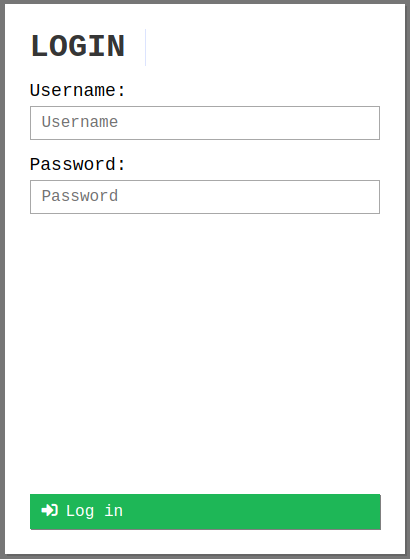
\includegraphics[width=0.95\linewidth]{InteraktionsDesign/Assets/Prototype/1.png}
            \caption{Login screen}
            \label{fig:prototype1}
        \end{figure}
    \end{minipage}
    \begin{minipage}{.33\textwidth}
        \begin{figure}[H]
            \centering
            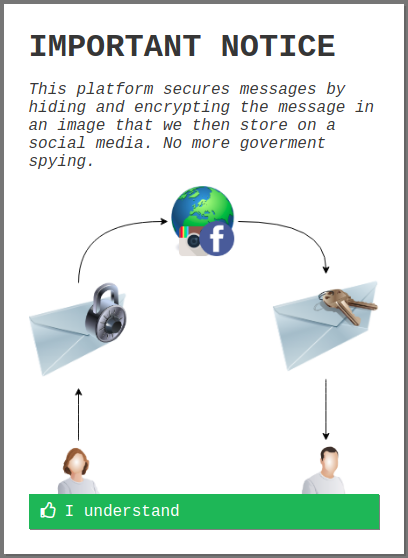
\includegraphics[width=0.95\linewidth]{InteraktionsDesign/Assets/Prototype/2.png}
            \caption{Main menu page}
            \label{fig:prototype2}
        \end{figure}
    \end{minipage}
    \begin{minipage}{.33\textwidth}
        \begin{figure}[H]
            \centering
            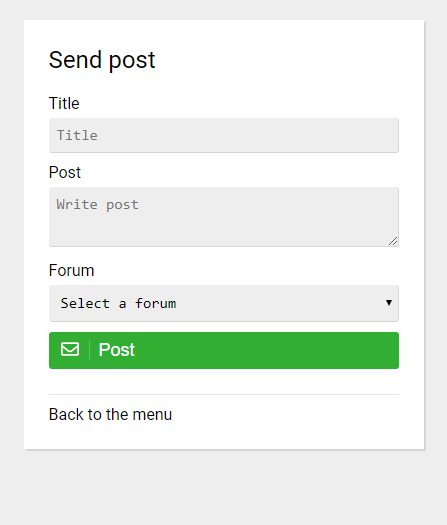
\includegraphics[width=0.95\linewidth]{InteraktionsDesign/Assets/Prototype/3.png}
            \caption{Send forum post}
            \label{fig:prototype3}
        \end{figure}
    \end{minipage}
    \begin{minipage}{.33\textwidth}
        \begin{figure}[H]
            \centering
            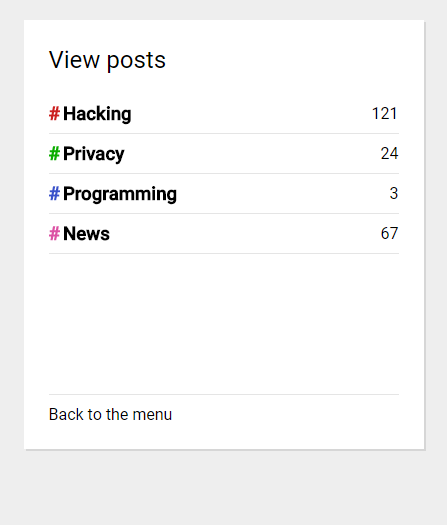
\includegraphics[width=0.95\linewidth]{InteraktionsDesign/Assets/Prototype/4.png}
            \caption{Forum overview}
            \label{fig:prototype4}
        \end{figure}
    \end{minipage}
    \begin{minipage}{.33\textwidth}
        \begin{figure}[H]
            \centering
            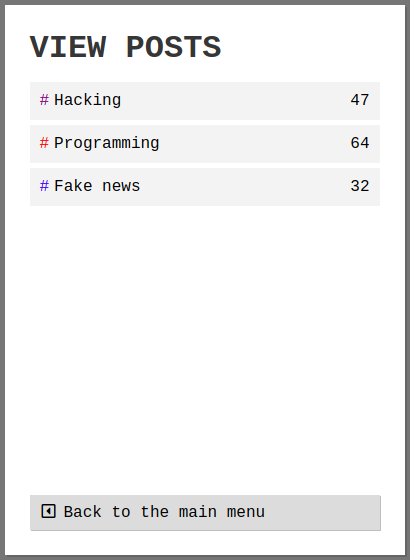
\includegraphics[width=0.95\linewidth]{InteraktionsDesign/Assets/Prototype/5.png}
            \caption{Forum post overview}
            \label{fig:prototype5}
        \end{figure}
    \end{minipage}
    \begin{minipage}{.33\textwidth}
        \begin{figure}[H]
            \centering
            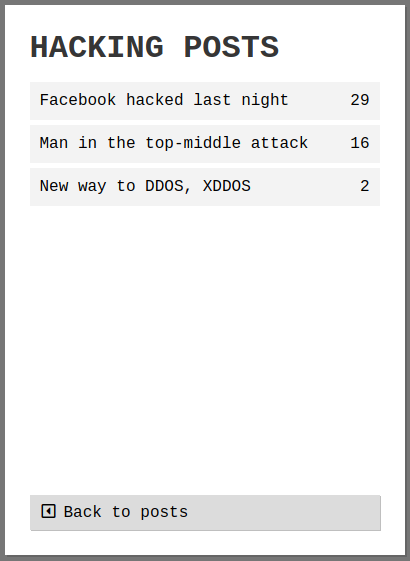
\includegraphics[width=0.95\linewidth]{InteraktionsDesign/Assets/Prototype/6.png}
            \caption{Inside a post}
            \label{fig:prototype6}
        \end{figure}
    \end{minipage}
    \label{fig:prototype}
\end{table}

The 6 images above show the most important pages in the application. It starts with the login screen [figure \ref{fig:prototype1}], where the user is prompted with the option to log into the system. The user is then greeted with a simple menu page, with the option to "Send post", "View posts" and "Logout" [figure \ref{fig:prototype2}]. If "Send post" is selected in the main menu, then a page with three inputs will appear [figure \ref{fig:prototype3}].